\documentclass[paperwidth=118cm,paperheight=84cm,landscape,fontscale=0.2941]{baposter}
%Dortes fontscale: 0.2941
\usepackage{lipsum} 
%841mm x 1189mm
\usepackage[font=small,labelfont=bf,hypcap=false]{caption} % Required for specifying captions to tables and figures
%\usepackage{cite}
\usepackage{booktabs} % Horizontal rules in tables
\usepackage{relsize} % Used for making text smaller in some places
%\usepackage[urlcolor  = blue]{hyperref}
%\graphicspath{{figures/}} % Directory in which figures are stored
\usepackage{multicol}
%\usepackage[style=ieee]{biblatex}
%\addbibresource{bib.bib}
\usepackage[utf8]{inputenc} 
%\usepackage{hyperref}
\usepackage{placeins}
\usepackage{epstopdf}
\usepackage{subcaption}
\usepackage[]{graphicx}
\usepackage{natbib}
\usepackage{times}

\usepackage[utf8]{inputenc}
\usepackage{fourier} 
\usepackage{array}
\usepackage{makecell}

\bibliographystyle{abbrvnat}

\selectcolormodel{RGB} %<-- Add colour model defintion
\definecolor{bordercol}{RGB}{255,255,255}%{33,26,82} % Border color of content boxes
\definecolor{headercol1}{RGB}{255,255,255}%{33,26,82} % Background color for the header in the content boxes (left side)
%\definecolor{headercol2}{RGB}{5,2,82} % Background color for the header in the content boxes (right side)
\definecolor{headerfontcol}{RGB}{0,0,0}%{255,255,255} % Text color for the header text in the content boxes
\definecolor{boxcolor}{RGB}{255,255,255} % Background color for the content in the content boxes

\begin{document}
\graphicspath{{Pictures/}}
\background{ % Set the background to an image (background.pdf)

}

\begin{poster}{
grid=false,
headerheight=0.14\textheight,
borderColor=bordercol, % Border color of content boxes
headerColorOne=headercol1, % Background color for the header in the content boxes (left side)
%headerColorTwo=headercol2, % Background color for the header in the content boxes (right side)
headerFontColor=headerfontcol, % Text color for the header text in the content boxes
boxColorOne=boxcolor, % Background color for the content in the content boxes
headershape=rectangle, % Specify the rounded corner in the content box headers
headershade=plain,
headerfont=\Large\sf\bf, % Font modifiers for the text in the content box headers
textborder=rectangle,
background=user,
headerborder=open, % Change to closed for a line under the content box headers
boxshade=plain,
eyecatcher=true
}
%
%----------------------------------------------------------------------------------------
%	TITLE AND AUTHOR NAME
%----------------------------------------------------------------------------------------
%
%\vspace{2em}
% Eye Catcher Images to go left of your title.
{

\includegraphics[height=0.10\textheight]{aau_logo_new.eps}
} %will not show if put eyecatcher=false
% Title
{\vspace{2pt}
Subjective Experience of Interacting with a Social Robot at a Danish Airport}
% Author
{
\vspace{3pt}
\normalsize{\textbf{Andreas Kornmaaler Hansen, Emil Bonnerup, Juliane Nilsson, Lucca Julie Nellemann \& Sara Nielsen}\\
Psychology Engineering - 17gr782 - Fall 2017 - School of Information and Communication Technology\\ Aalborg University, Aalborg, Denmark\\ }
$\{$akha14, ebonne14, jnils12, ljne14, snie14$\}$@student.aau.dk\\
}
{

\includegraphics[height=0.10\textheight]{aau_logo_new.eps}
}

%----------------------------------------------------------------------------------------
%	INTRODUCTION
%----------------------------------------------------------------------------------------
\headerbox{Introduction}
{name=introduction,column=0,row=0, span=1}
{\parskip 5pt   
This study originates from a social robot research project at Aalborg University with the aim of developing and implementing robots in a variety of contexts. This raises questions as to how social robots should behave and which variables are important when implementing a social robot in a public setting. Important variables can be elicited via user interaction and tested via scales. The study consists of two tests, one where variables are elicited and one where the scales are used to evaluate the experience the human robot interaction (HRI). %, so possible correlation can be detected.  
}

\headerbox{Methods}
{name=method,span=1,column=0,below=introduction, span=1}
{\parskip 5pt 
Two tests were set up in Aalborg Airport (AAL) to investigate which variables are important for the HRI with a social robot and to develop scales based on them. Both tests were conducted on Danish Travellers who interacted with a \textit{Double} robot shown on figure 1.\\
\textbullet~ \textbf{Subject recruitment} was done by the robot which approached potential subjects (travellers) and presented a wireframed interface asking if it may help with wayfinding. If the traveller accepted  they were led towards their chosen destination until an experimenter stopped them. The \textit{Double} robot was remotely controlled via a computer by a present researcher. This approach was similar in both tests and was done to provide a more ecological and undisturbed interaction between robot and subject.\\
\textbullet~ \textbf{Test 1}: Subjects were asked to participate in a semi-structured interview about their first impressions after the interaction while observational data was gathered during the interaction. \\
\textbullet~ \textbf{Test 2}: Subjects were asked to rate their interactions on the developed scales on a PC after their unsolicited interaction.
%In the first test subjects were asked to participate in a semi-structured interview about their first impressions after the interaction and in the second test subjects were asked to rate their interactions on the developed scales. The \textit{Double} robot was remotely controlled via a computer and a present controller. On the screen a developed wireframe to help with wayfinding in AAL was presented. 
\vspace{-11pt}  

\begin{center}
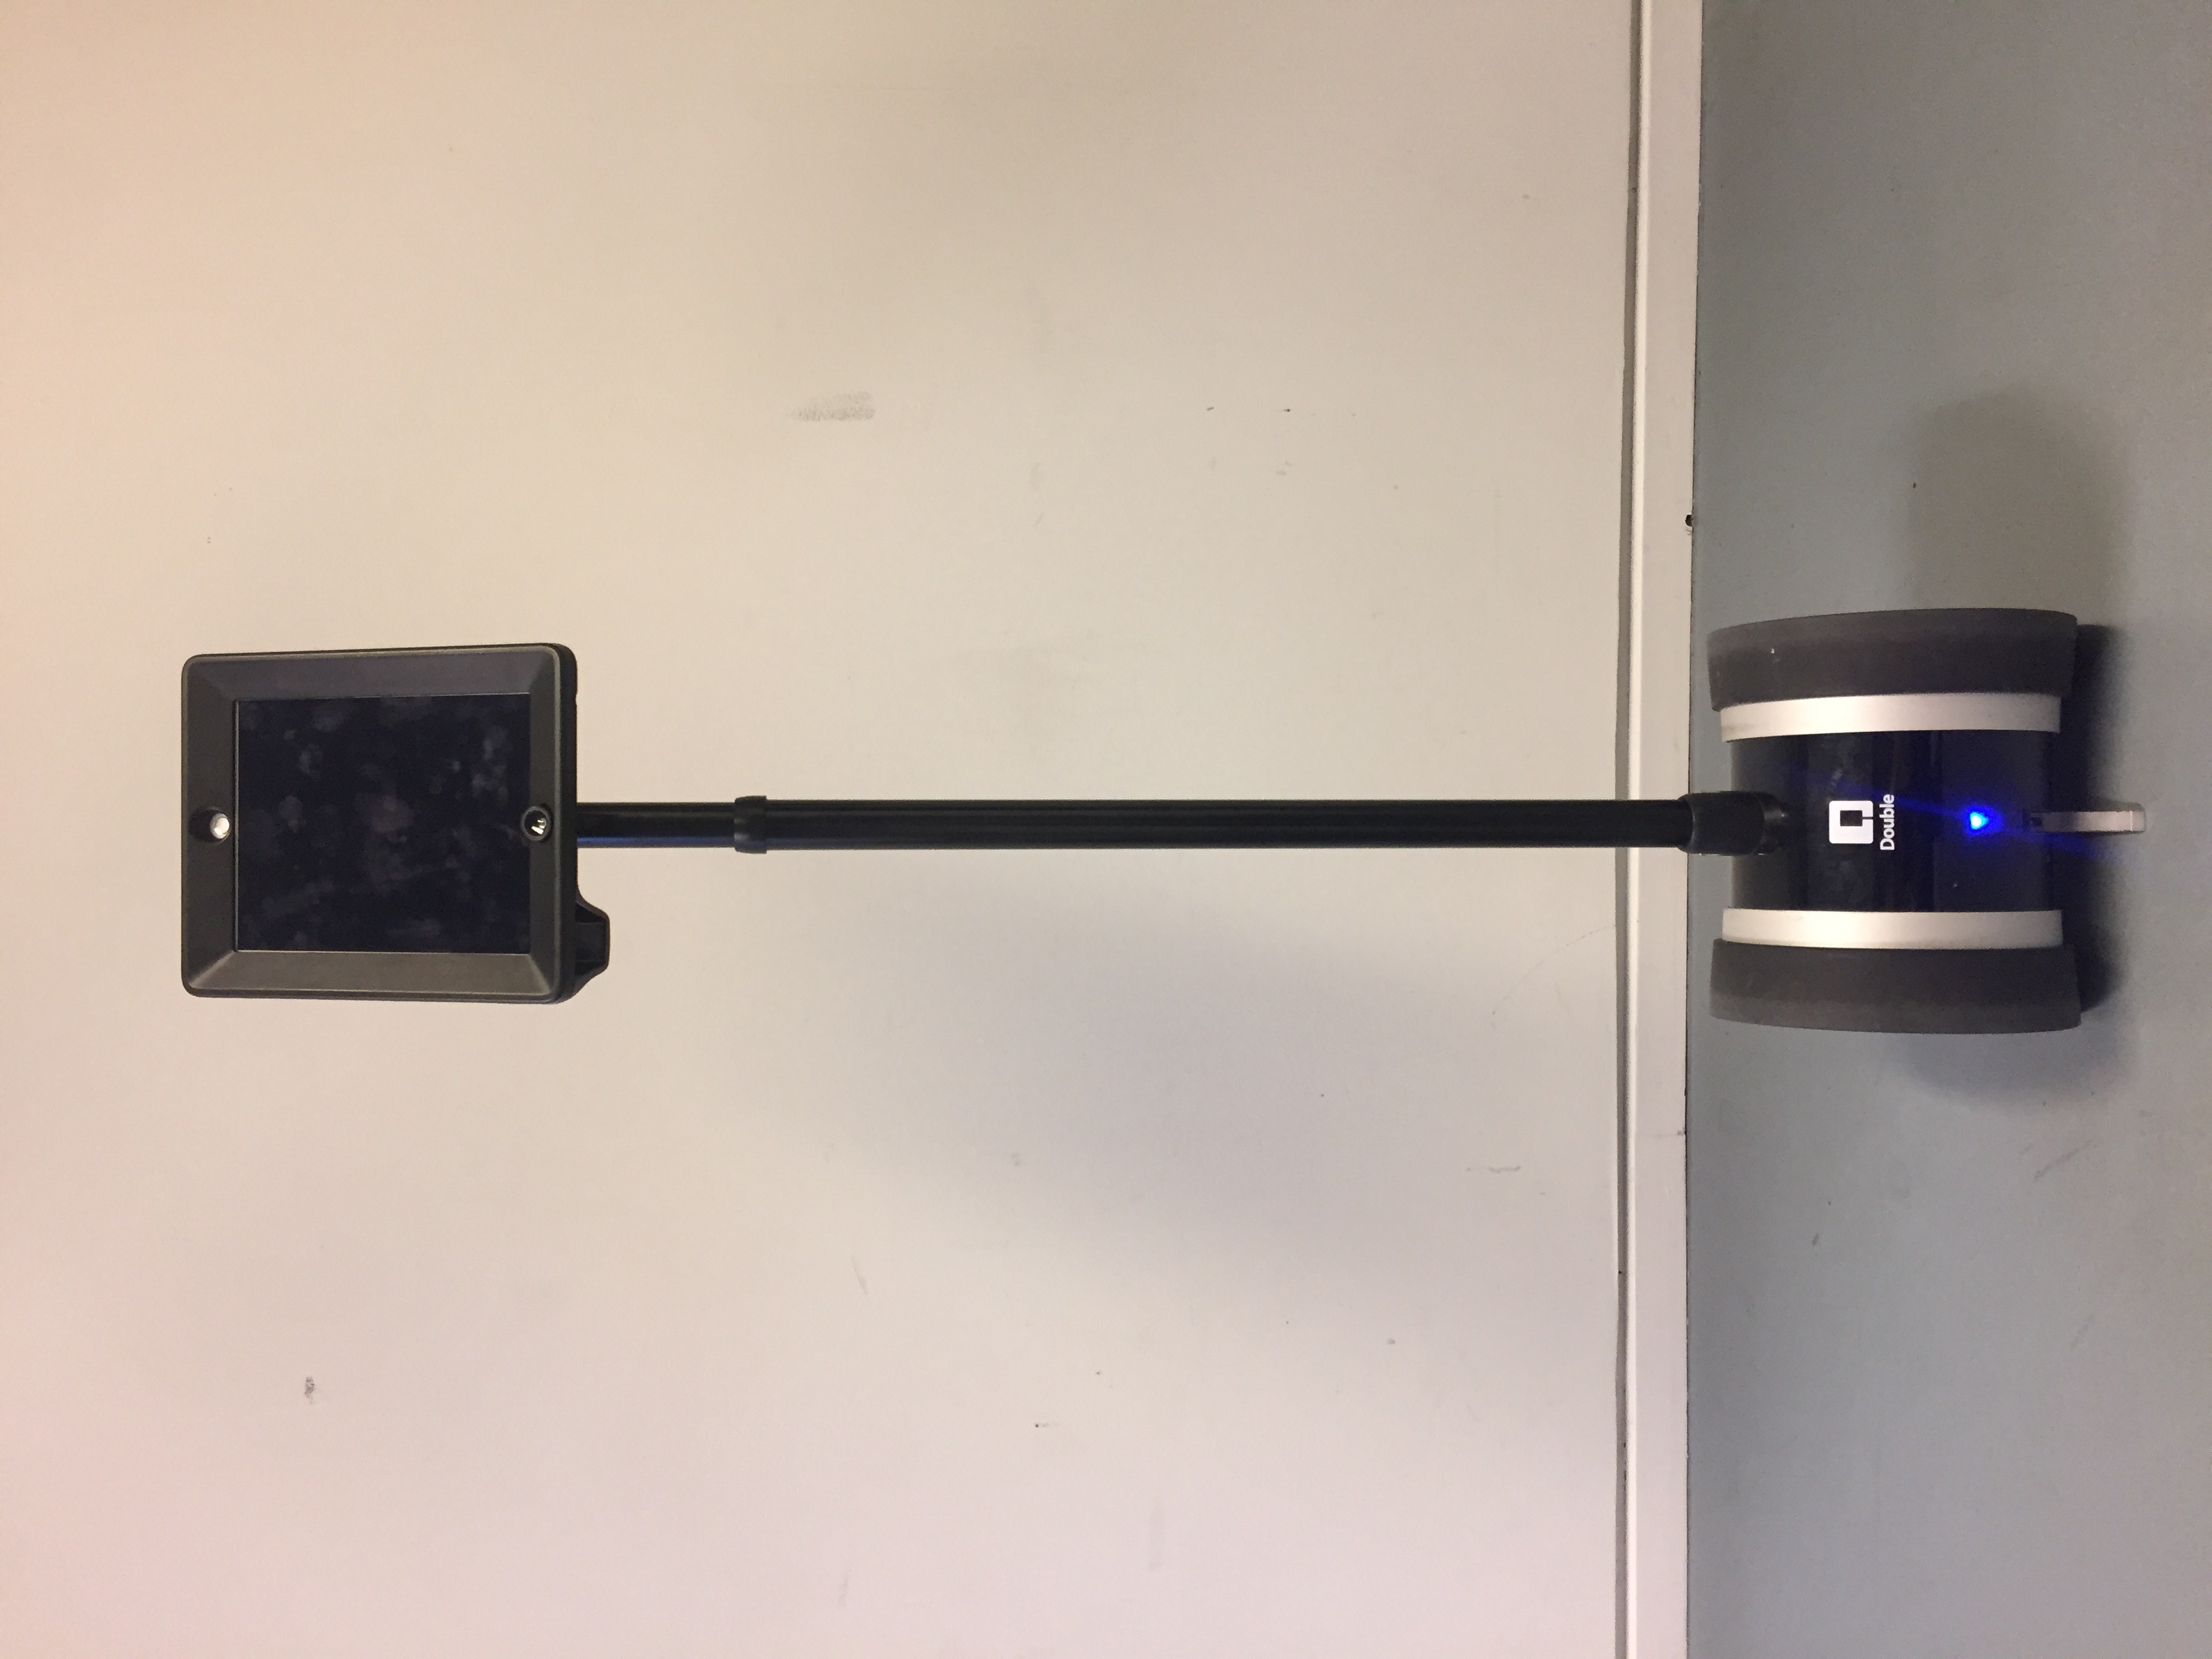
\includegraphics[width=0.40\linewidth]{ModificeretDoubleFront.eps}
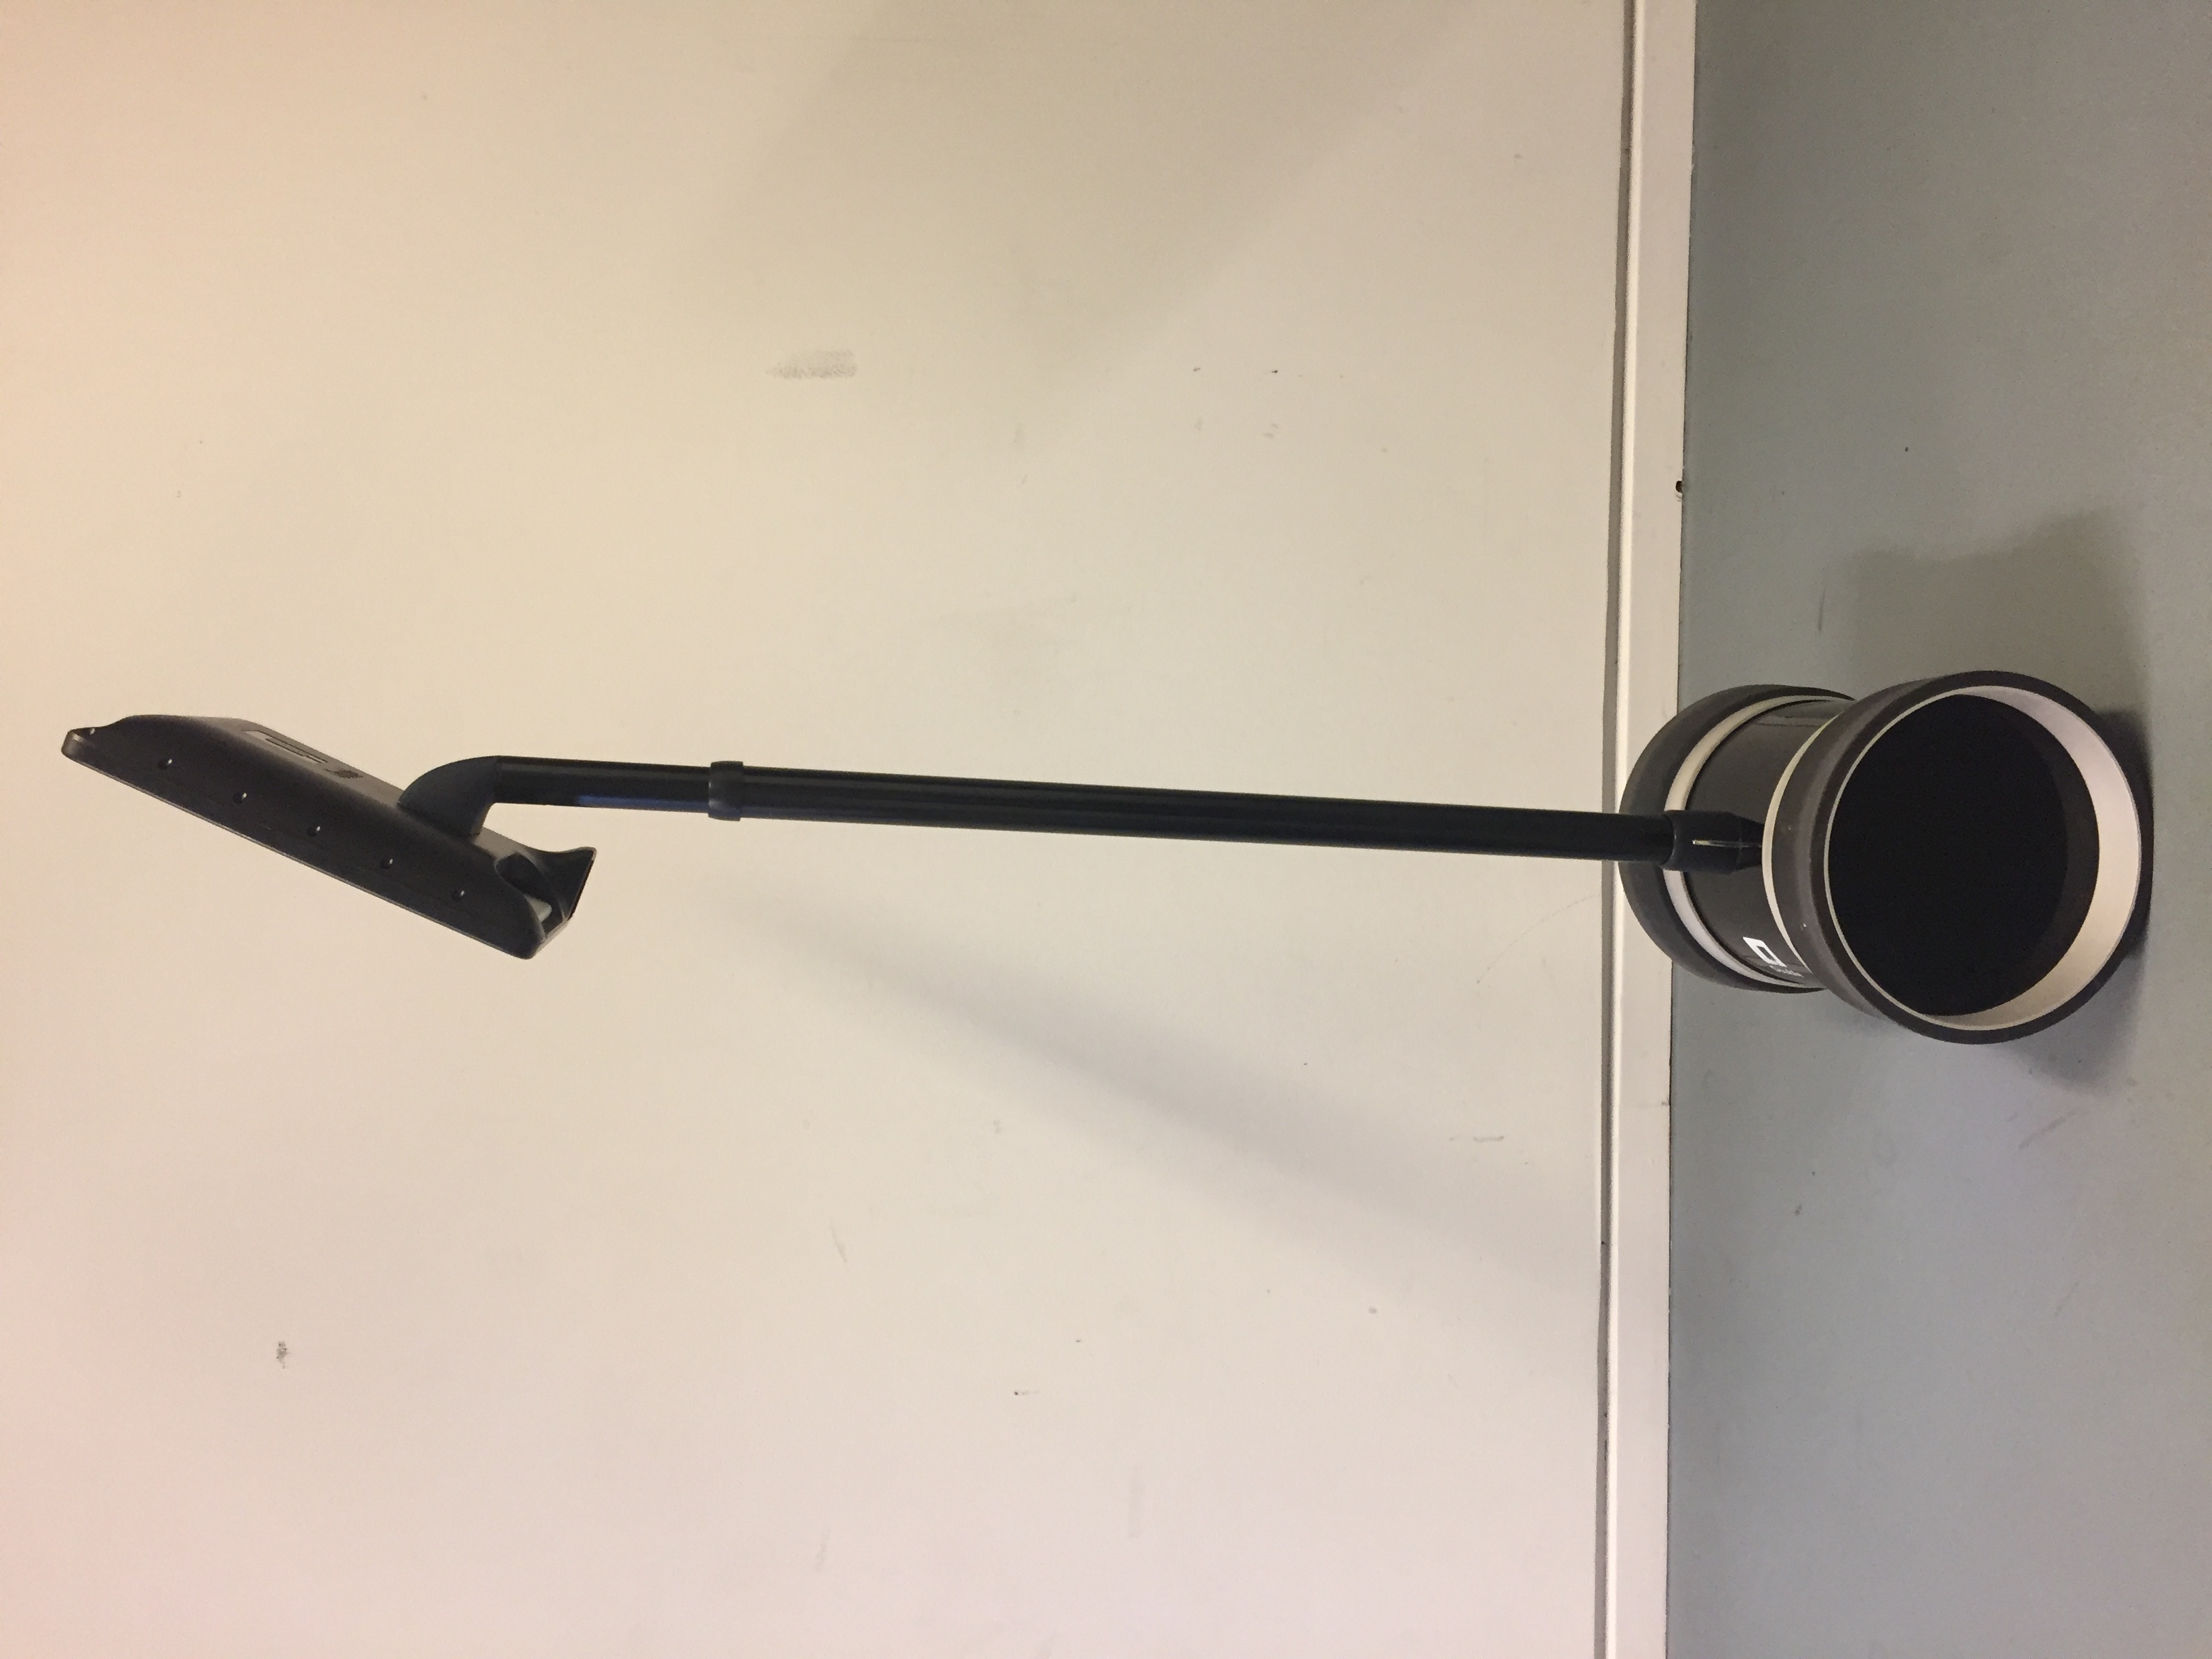
\includegraphics[width=0.40\linewidth]{ModificeretDoubleSide.eps}

\textbf{Figure~1. }\textit{Double}'s front and profile.
\end{center}
\vspace{-15pt}  

%The subjects were recruited by the robot, which provides a more ecological and undisturbed interaction between robot and subject. The robot approached potential subjects after the security check and asked to help travellers with wayfinding. If travellers wanted help, they were presented with four wayfinding options: Food, Shopping, Toilets or Gate information. After the interaction the robot led subjects to an interviewer. 

%\textbullet~ \textbf{Data Processing}
%From the first test the interviews and observations were coded into affinity notes and an affinity diagram was made. This affinity diagram is pivotal in eliciting the variables that affect HRI, and thereafter in creating the scales to be used for further work. 
%567 affinity notes were sorted into 10 green categories with individual subcategories. 

%From the second test \textbf{Beskriv kort den databehandling samt vi gerne vil finde mulige korrelationer mellem skalaer}
}


\headerbox{Results - Elicitation of variables}
{name=results1,span=1,column=1,aligned=introduction, span=1}
{\parskip 5pt 
From the first test an affinity diagram was made, see figure 2, where one of the 10 categories are shown.
\vspace{-10pt}  
\begin{center}
	\includegraphics[width=0.7\linewidth]{Affinity.eps}
	
	\textbf{Figure~2. }The category, approach, from the developed affinity diagram.
\end{center}
\vspace{-10pt}  
24 variables were elicited, where 23 of them are used to evaluate the HRI and one is used as demographic information about subjects. All 24 variables are evaluated on a Visual Analogue Scales (VAS). The 23 used to evaluate the interaction is shown on figure 2.
  
%\begin{itemize}
%	\setlength\itemsep{-2em}
%	\item SQ1: How do think the screen on the robot reacted? (S1)\\
%	\item SQ2: How did you experience the robot? (S2)\\
%	\item SQ3: How was it to use the robot? (S3)\\
%	\item SQ4: How did you experience the robot's movements? (S4) \\
%	\item SQ5: I think that the robot stopped... (S5)\\
%	\item SQ6: I think that the robot's speed is... (S6)\\
%	\item SQ7: I think that the robot's height is... (S7)\\
%	\item SQ8: I feel that the robot can help me (S8-S13)\\
%	\item SQ9: I think that the robot was obstructing me (S8-S13)\\
%	\item SQ10: I feel safe around the robot (S8-S13)\\
%	\item SQ11: The robot startled me (S8-S13)\\
%	\item SQ12: I like to be served by the robot (S8-S13)\\
%	\item SQ13: I counted on the robot to lead me to the location I chose (S8-S13)\\
%	\item SQ14: How personal did you experience the robot's help? (S14)\\
%	\item SQ15: How surprised were you by the robot's approach? (S15)\\
%	\item SQ16: What do you think about the robot? (S16-S19)\\
% 	\item SQ17: What else do you think about the robot? (S20-S23)\\\vspace{-15pt}
%\end{itemize}

\vspace{-15pt}
\begin{center}
	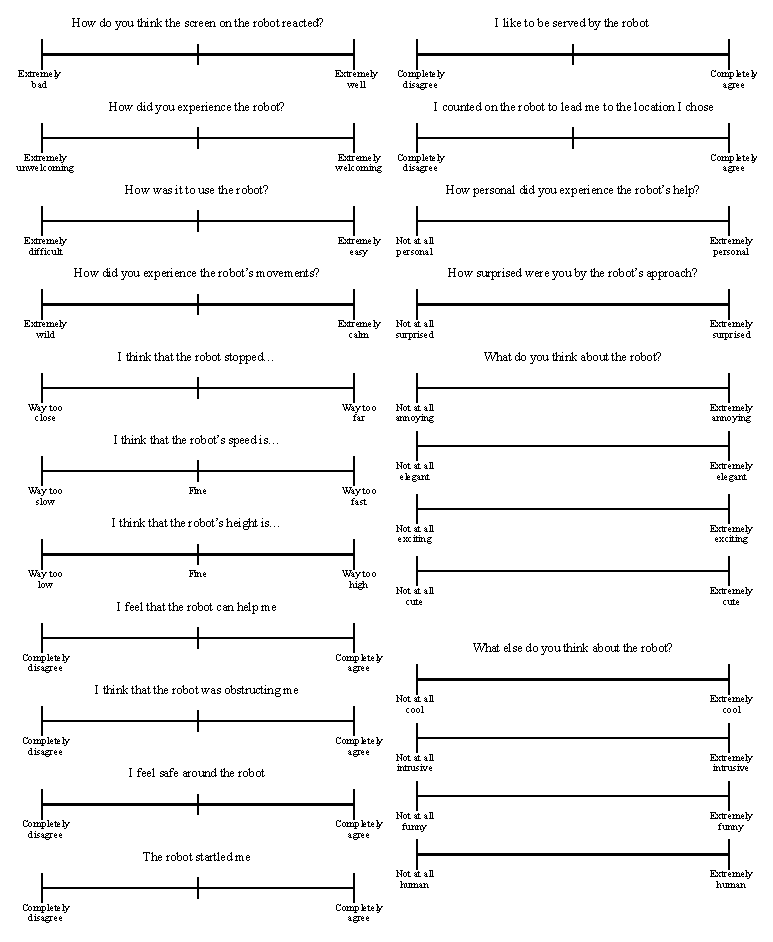
\includegraphics[width=1.0\linewidth]{AllScalesSpace.eps}

\textbf{Figure~3. }The 23 VAS developed from the elicitated variables.
\end{center}
\vspace{-15pt}

The 24th variable has the scale question "How fond of technology are you?" and is evaluated on a unipolar VAS with anchor points: \textit{Not at all fond} and \textit{Extremely fond}.
}



\headerbox{Results - Scale Testing}
{name=results2,span=1,column=2,aligned=introduction}
{\parskip 5pt
\begin{center}
%	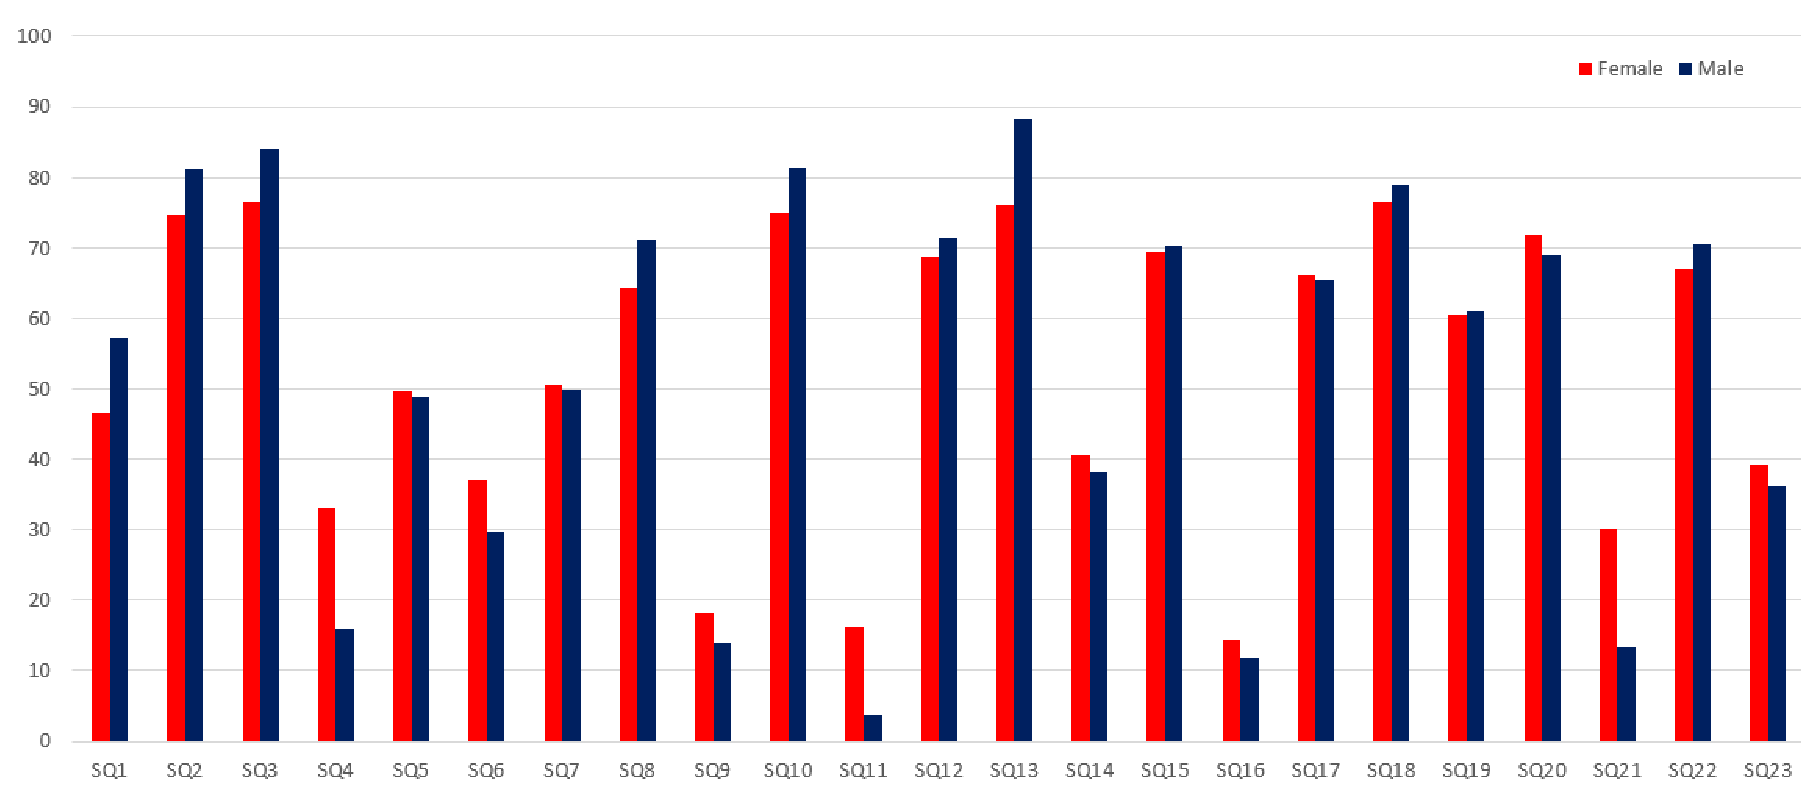
\includegraphics[width=1.0\linewidth]{KoenGennemnitligBesvarelser.eps}

%\textbf{Figure~3. }The three types of VAS developed from the elicitated variables.
\vspace{-10pt}
	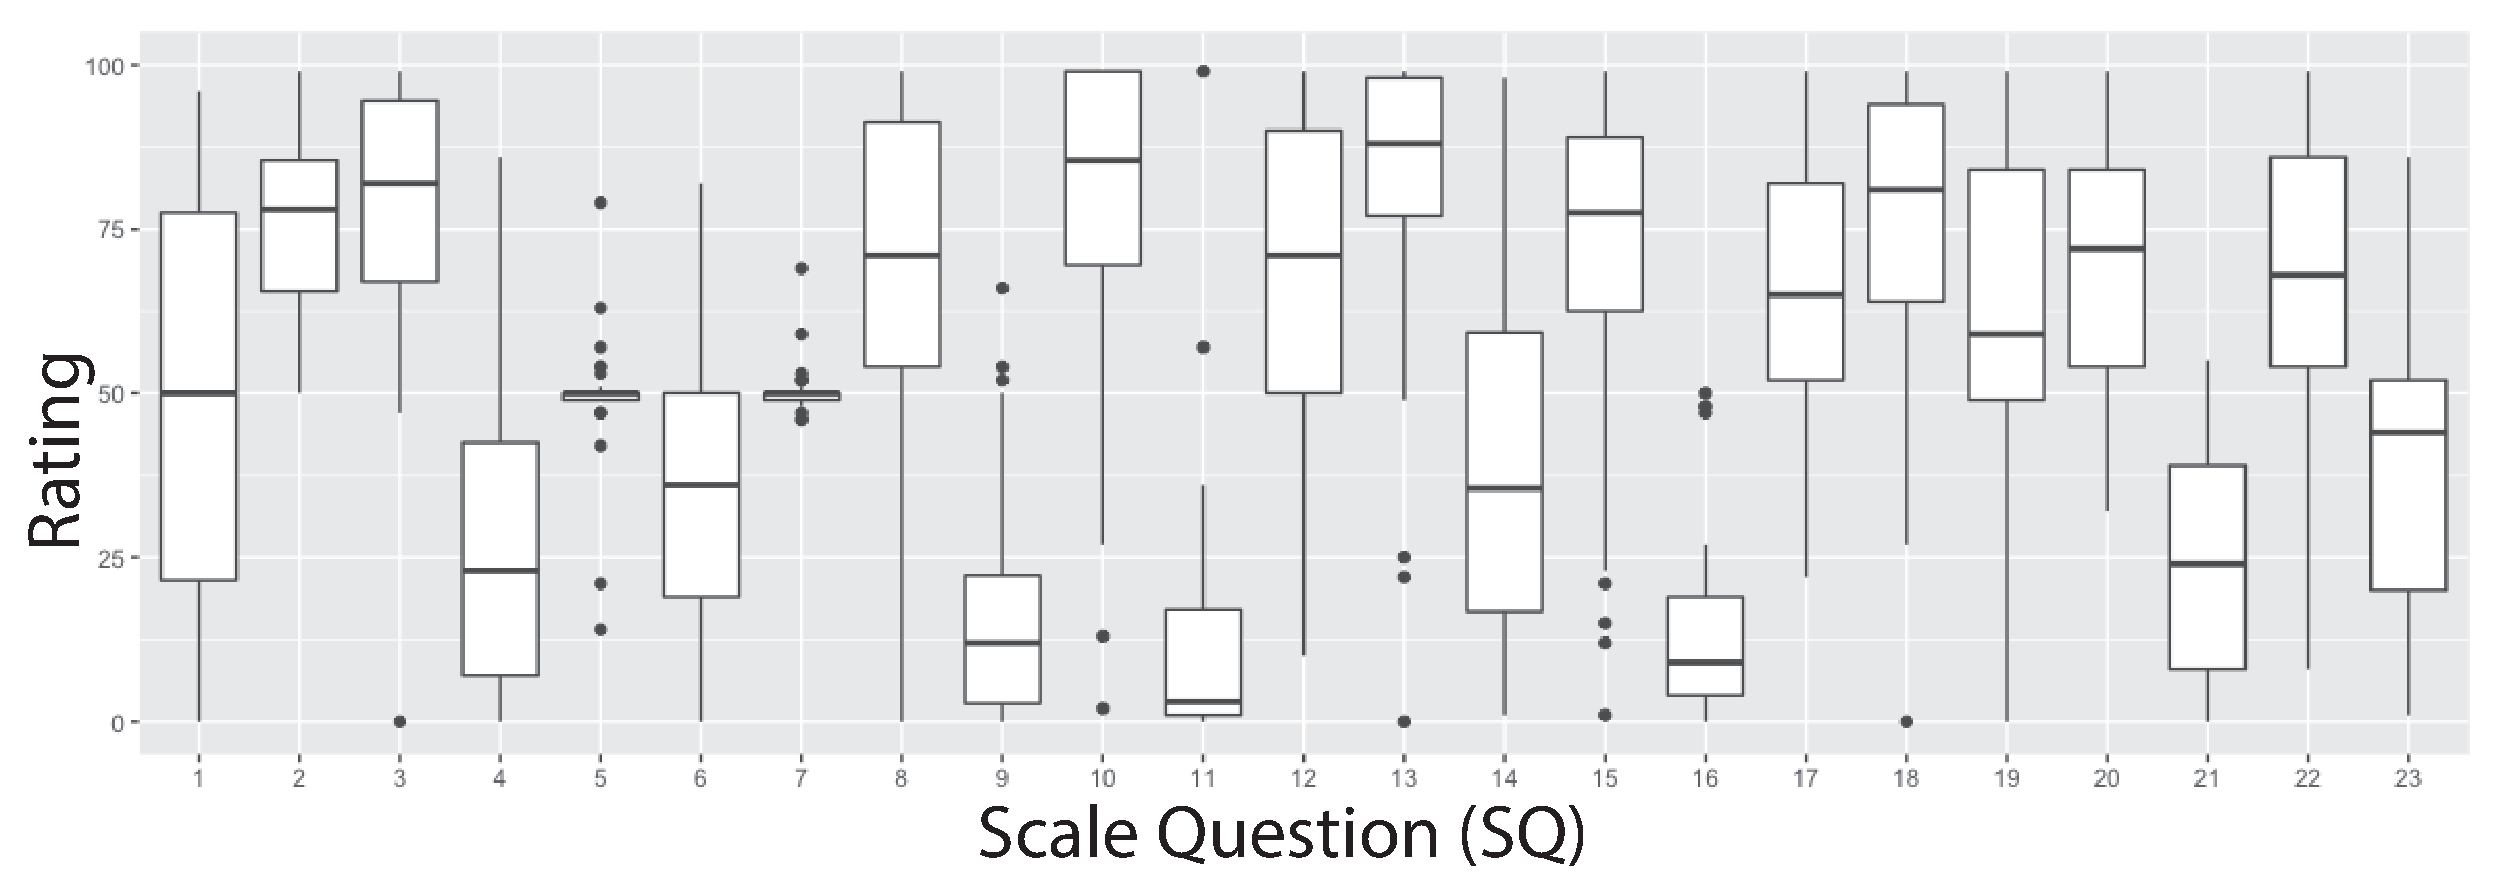
\includegraphics[width=0.1\linewidth]{Boksplot0er.eps}

\textbf{Figure~4. }Boxplot based on the rating from answers on the 23 scales. SKRIV HVAD TINGENE VISER

	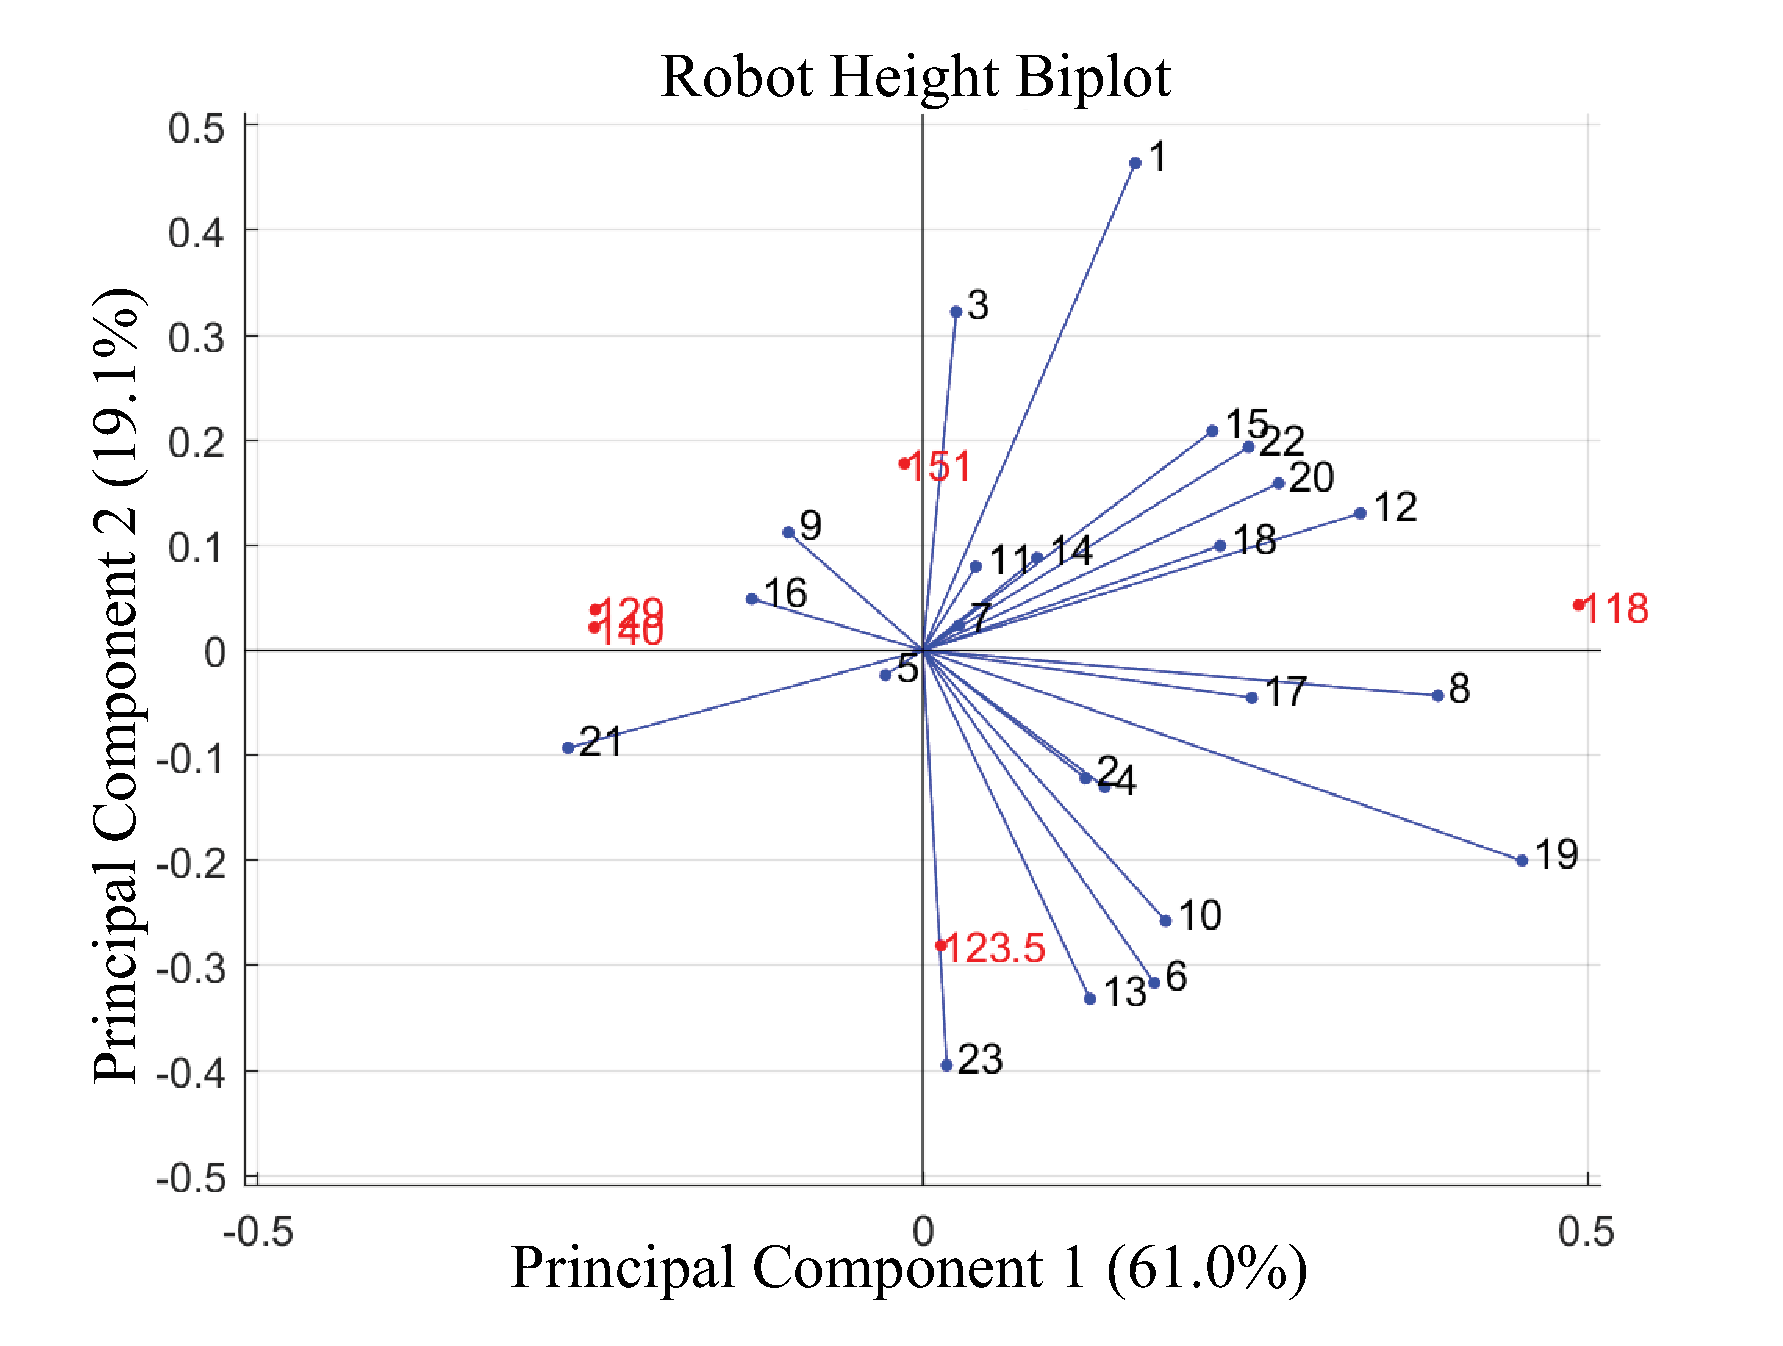
\includegraphics[width=0.9\linewidth]{RHeight-Biplot.eps}
	\vspace{-10pt}
	
\end{center}
\textbf{Figure~5. }Biplot showing how the different variables contributes to components and which variables correlates. The black numbers relates the the SQ and the red to the different heights.


From the biplots, the first bulletpoint is variables that correlates positive and the second is variables that correlates negative when doing PCA related to heights:

\textbullet~SQ10-SQ13, SQ12-SQ18, SQ14-SQ15, SQ8-SQ17\\
\textbullet~ SQ12-SQ21, SQ18-SQ21, SQ2-SQ9, SQ4-SQ9, SQ16-SQ19

The same apply wheen doing PCA related to distance:

\textbullet~SQ1-SQ12, SQ7-SQ17, SQ10-SQ22, SQ8-SQ21\\
\textbullet~ SQ2-SQ9, SQ14-SQ16, SQ10-SQ13, SQ13-SQ22, SQ5-SQ21, SQ19-SQ20


The same apply wheen doing PCA related to direction:

\textbullet~SQ8-SQ10, SQ9-SQ14, SQ5-SQ7\\
\textbullet~ SQ1-SQ12, SQ9-SQ10, SQ10-SQ14, SQ6-SQ23, SQ13-SQ21


%\vspace{-15pt}


	


}


\headerbox{ }
{name=results3,span=1,column=3,aligned=introduction}
{\parskip 5pt
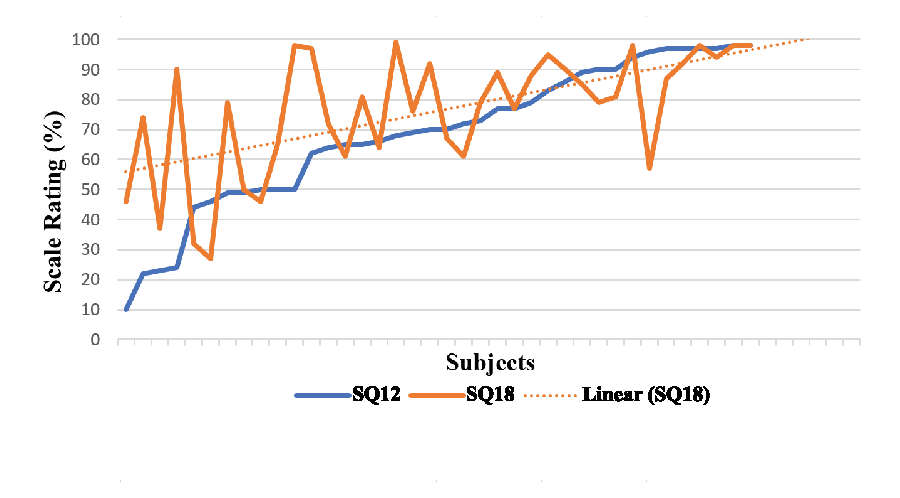
\includegraphics[width=0.9\linewidth]{SQ12_SQ18.eps}

\textbf{Figure~5. }The three types of VAS developed from the elicitated variables.
}

\headerbox{Conclusion}
{name=conclusion,span=1,column=3,below=results3}
{\parskip 5pt
This research conducted in this study reveals that there are at least 23 variables that Danish travellers find important when interacting with a social robot. 


}


\headerbox{Acknowledgements}
{name=akn,span=1,column=3,below=conclusion}
{\parskip 5pt
The authors would like to thank Karl Damkjær Hansen, postdoc at Aalborg University, for suggesting this study, giving professional insights and feedback, helping with technical support, and lending the \textit{Double} robot to the authors.
The authors would also like to thank Professor Dorte Hammershøi for supervising the study. 
Last the authors would like to thank Aalborg Airport for providing access to the wanted user group and facilities by letting the authors conduct their field studies at the airport. 
}


\headerbox{Key references}
{name=references,column=3,below=akn}
{
\renewcommand{\section}[2]{}%
%\parskip 5pt
 %   \bibliography{bib.bib}
%\tiny
\footnotesize
%Dorte har skrevet kilder ind på følgende måde
%Abdala C (1996) JASA \textbf{100}(6):3726-3740.
%Bonfils P et al. (1991) \textit{Arch Otolaryngol Head Neck Surg} \textbf{117}(10):1167–1171.
%Brown DK et al. (2000) \textit{Hearing Res}. \textbf{145}(1-2):17-24.
}


%-------------------------------------------------------------------------

\end{poster}
\end{document}